\documentclass{beamer}
\usepackage{algorithmic}
\usepackage{multimedia}

\usetheme{default}

\setbeamercolor{umbcboxes}{bg=violet!12,fg=black}

\usepackage{rotating} % for defining \schwa
\newcommand{\schwa}{\raisebox{1ex}{\begin{turn}{180}e\end{turn}}}

\newcommand{\arcsinh}{\mathop\mathrm{arcsinh}\nolimits}
\newcommand{\arccosh}{\mathop\mathrm{arccosh}\nolimits}
\newcommand{\Pu}{P_{\mathrm{amb}}}

\title{Path-Selection in Floating Sensor Networks}
\author[K. Weekly]{Kevin Weekly}
\institute[UCB]{
  Dept. of Electrical Engineering and Computer Sciences\\
  University of California, Berkeley \\
}
\date{April 15, 2011}

\begin{document}
\begin{frame}[plain]
  \titlepage
\end{frame}


\begin{frame}{Outline}
\begin{enumerate}
  \item Problem setup
 \begin{itemize}
  \item Link Labelling
  \item Path enumeration
  \item Path/Region costs
 \end{itemize}

  \item \{0,1\} Linear Programs
  \begin{itemize}
  \item General Formulation
  \item All links minimum units
  \item Maximum coverage fixed units
  \end{itemize}

  \item Mixed Integer Quadratic Programs

\end{enumerate}
\end{frame}


\begin{frame}{Problem Setup: Link Labelling}
Breadth-First-Search (BFS) style flood-fill:
\begin{itemize}
   \item Maintains edge list of water pixels to process and processes them in BFS order.
   \item Each edge is given a label. As it sweeps through the domain, that label is assigned to underlying pixels.
   \item Monitors continuity of edges.
\begin{itemize}
    \item Path Splitting: If a previously continuous edge becomes broken, two new labels are generated and connections are recorded. 
    \item Path Joining: If two edges meet, a new label is generated and connections are recorded.
\end{itemize}
   \item Algorithm ends when there are no more water pixels to process.
\end{itemize}

\end{frame}

\begin{frame}{Problem Setup: Link Labelling}

\begin{figure}
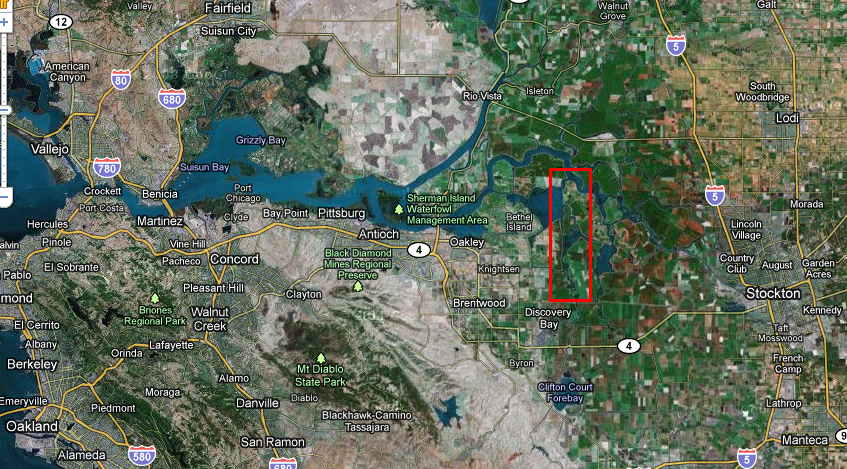
\includegraphics[width=0.55\linewidth]{figures/domain.png}\\
\movie[width=0.2\linewidth, height=0.5\textheight, rate=2, autostart, repeat, poster]{}{figures/anim_edge.mpg}
\movie[width=0.2\linewidth, height=0.5\textheight, rate=2, autostart, repeat, poster]{}{figures/anim2.mpg}
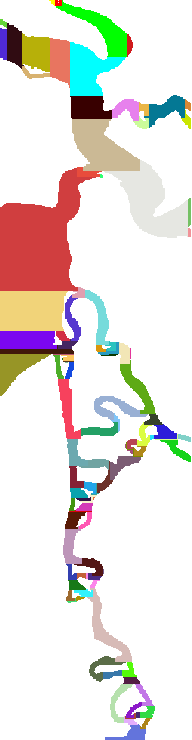
\includegraphics[height=0.5\textheight]{figures/labelled.png}
\end{figure}

\end{frame}


\begin{frame}{\{0,1\} Linear Programs: Static Formulation}
\begin{align*}
\max_{x,y}\;& -g^Tx + h^Ty \\
\mbox{s.t.}\;& \left[ \begin{array}{c}
                       A\\
                       -1, \dots, -1
                      \end{array}\right] x \geq \left[ \begin{array}{c} y\\-D \end{array}\right] \\
&a_{ij} = \begin{cases}
           1\;\mbox{if path $i$ contains link $j$}\\
           0\;\mbox{otherwise}
          \end{cases}\\
&x_i \in \{0,1\}\;\forall i\in\{1\dots n\}\\
&y_i \in \{0,1\}\;\forall i\in\{1\dots m\}
\end{align*}

\begin{itemize}
\item $\{x_i\}$ : indicates whether path $i$ of $n$ total paths is taken.
\item $\{y_j\}$ : indicates whether link $j$ of $m$ total links is visited.
\item $D$ : total number of units avaiable.
\item Preprocessing step : Remove all links impossible to visit (zero-rows of A).
\end{itemize}

\end{frame}


%%%%%%%%%%%%%%%%%%%%%% ALL LINKS MINIMUM UNITS %%%%%%%%%%%%%%%%%%%%%%%%%%%%%%%%%%%%%%%%%%%%%%
\begin{frame}{\{0,1\} Linear Programs: All links minimum units}
\emph{``Visit every link using the least number of drifters''}
\begin{align*}
g &= \left[ 1,1, \dots ,1\right]\\
y &= \left[ 1,1, \dots ,1\right]\\
D &= \infty \;\mbox{(remove row from ILP)}
\end{align*}

\begin{itemize}
 \item Preprocessing : Find paths which must be taken ( rows of A containing only one 1 ). Remove these paths and all of their links from ILP. Repeat until all rows of A have two or more 1s.
\end{itemize}
\end{frame}

\begin{frame}{\{0,1\} Linear Programs: All links minimum units}
\begin{figure}
  \begin{tabular}{|l|c|}
  \hline 
  Paths in ILP/Total & 1544/1547 \\
  Labels in ILP/Total & 70/105 \\
  CPU Time (cplex) & 250mS\\
  CPU Time (glpk) & 180mS \\
  Units Needed & 10 \\
  \hline
  \end{tabular}
\end{figure}

  \begin{figure}
     {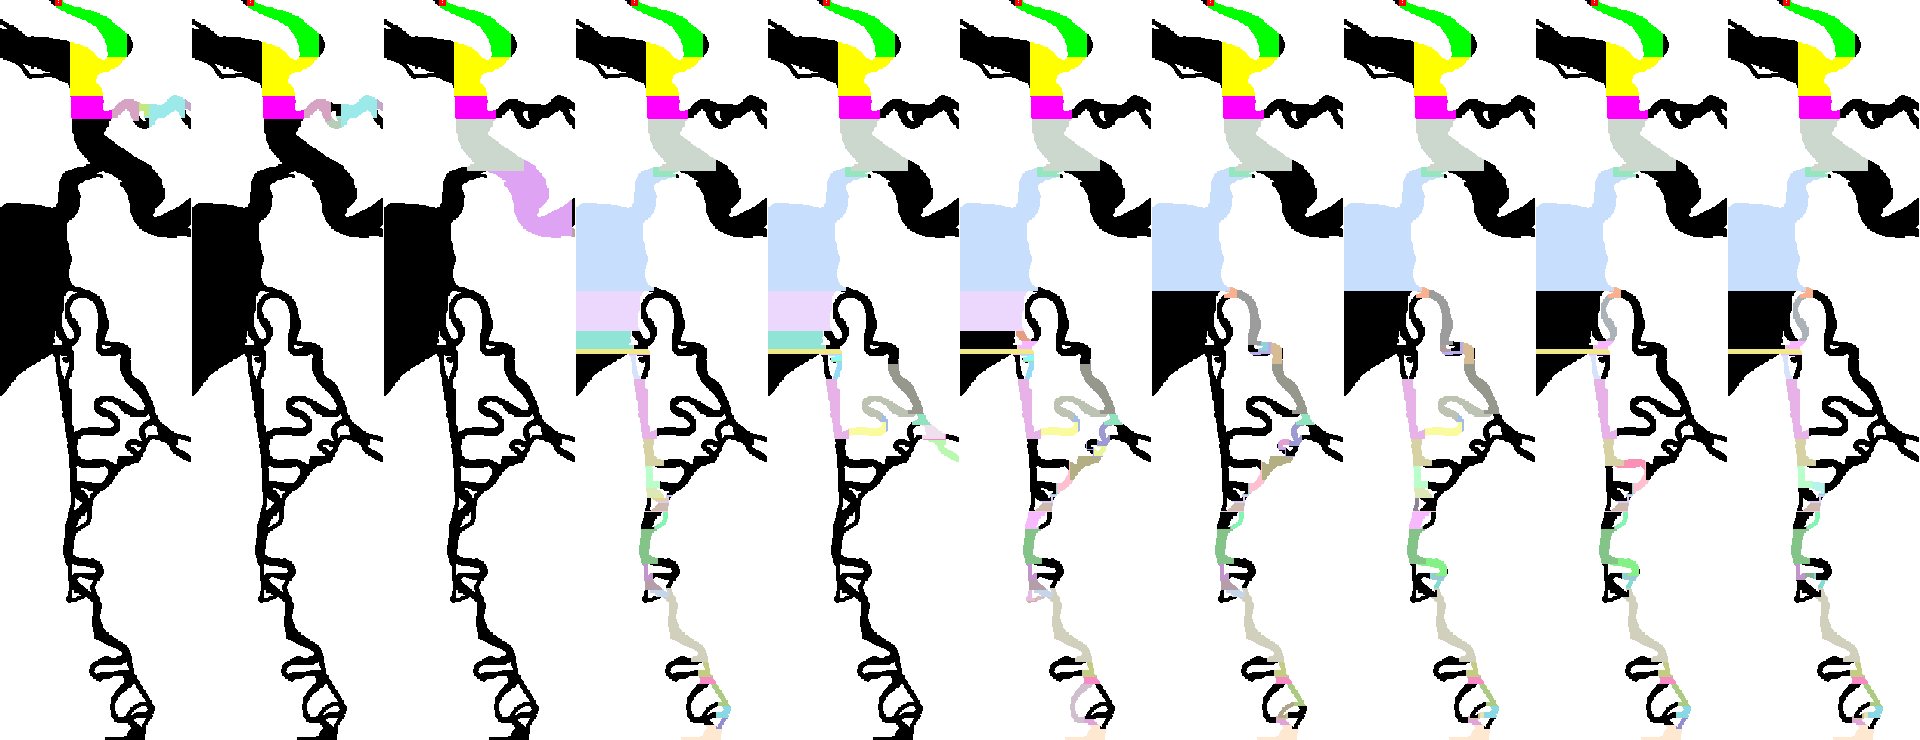
\includegraphics[width=1\textwidth]{figures/all_links_minimum_units_paths.png}}
  \end{figure}
\end{frame}


%%%%%%%%%%%%%%%%%%%%%% MAX COVERAGE FIXED UNITS %%%%%%%%%%%%%%%%%%%%%%%%%%%%%%%%%%%%%%%%%%%%%
\begin{frame}{\{0,1\} Linear Programs: Max coverage fixed units}
\emph{``Visit the greatest total weighted area with a fixed number of units.''}
\begin{align*}
g &= 0\\
h &= \left[ w_1,w_2, \dots ,w_m\right]\\
D &= 5\\
\end{align*}

\begin{itemize}
 \item Path processing : Set $w_j$ to the weight of each region with label $j$.
 \item Note: Setting $w_j=1$ solves the problem\\ \emph{``Visit the most number of links with a fixed number of units.''}
\end{itemize}
\end{frame}

\begin{frame}{\{0,1\} Linear Programs: All links minimum units}
Example: $w_j$ are the number of pixels in each region.
\begin{figure}
  \begin{tabular}{|l|c|}
  \hline 
  Paths & 1547 \\
  Labels in ILP/Total & 82/105 \\
  CPU Time (cplex) & 440mS\\
  CPU Time (glpk) & 210mS \\
  Pixels covered/Total & 31169/36514 (85\%)\\
  \hline
  \end{tabular}
\end{figure}

  \begin{figure}
     {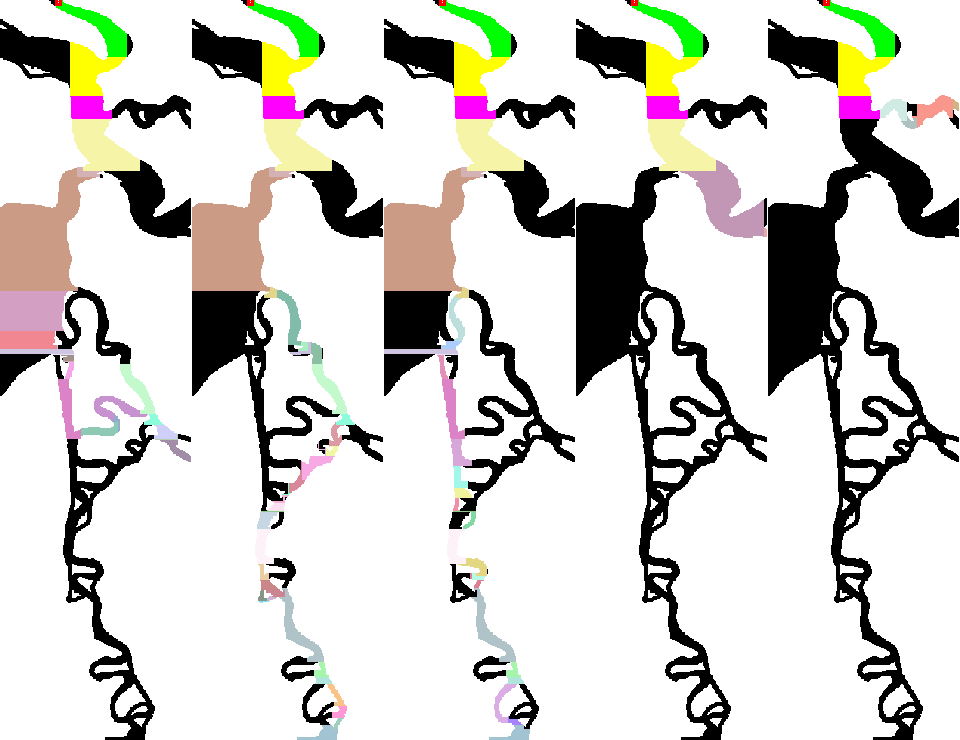
\includegraphics[width=0.5\textwidth]{figures/max_coverage_fixed_units_paths.png}}
  \end{figure}
\end{frame}


\end{document}